\chapter{LibreLogo} \label{cap:librelogo}

LibreLogo è l'unione del celebre programma Logo e il \textit{word} \textit{processor} Writer, che è l'equivalente di Word. Word fa parte della ben nota \textit{suite} Microsoft Office mentre Writer fa parte di LibreOffice, che è software libero. Logo è stato creato negli anni 70 da Seymour Papert per facilitare l'insegnamento della matematica mediante il computer. Seymour Papert è un matematico nato in Sudafrica nel 1928., ha studiato matematica a Johannesburg e poi a Cambridge. Ha fatto ricerca in una varietà di luoghi fra cui l'università di Ginevra, fra il 1958 e il 1963. È in questo periodo che ha lavorato con Jean Piaget, diventando uno dei suoi collaboratori preferiti – interessante connubio fra un matematico e un pedagogista. Nel 1963 è stato ricercatore presso il MIT (Massachusetts Institute of Technology) dove, nel 1967, è stato nominato codirettore del celebre MIT Artificial Intelligence Laboratory dal direttore fondatore, Marvin Minsky. Lo stesso laboratorio dove pochi anni dopo avrebbe operato Richard Stallman, ideatore del concetto di software libero e autore dei primi fondamentali componenti software su cui, negli anni '90, si sarebbe basato il software operativo Linux.  Papert è famoso per avere inventato Logo, un linguaggio che consente di creare grafica manovrando il movimento di una “tartaruga” mediante opportuni comandi. Nella prima versione, ideata negli anni '70, la tartaruga era in realtà un robot che disegnava mentre si muoveva.
\begin{figure}
   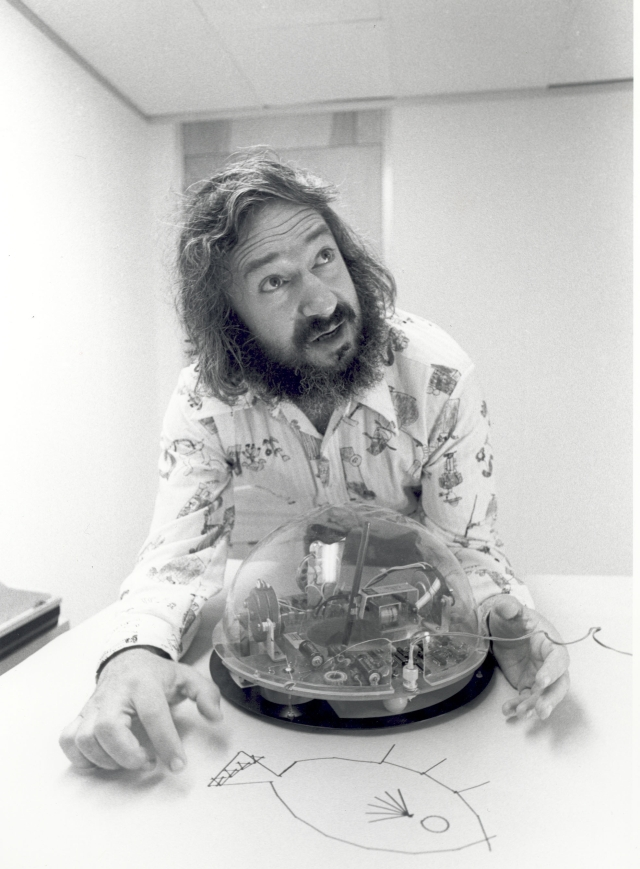
\includegraphics[width=10.0cm]{./images/librelogo/Papert-x640.jpg}
   \caption{Seymour Papert mostra una delle prime versioni di Logo, quando era ancora un vero e proprio robot per disegnare.} 
\label{papert}
\end{figure}
Quando i computer arrivarono nelle case, negli anni '80, Logo divenne un software e come tale è stato descritto da Seymour Papert  in \textit{Mindstorms}. Per capire la valenza pedagogica del pensiero di Papert leggiamo questo brano, tratto proprio da \textit{Mindstorms} (pp. 7-8) \cite{Papert}:

\begin{quote}
Da Piaget prendo il modello del bambino come costruttore delle proprie strutture mentali. I bambini hanno il dono innato di imparare da soli e sono in grado di assumere un'enorme quantità di conoscenza grazie a un processo che io chiamo “apprendimento piagetiano”, o “apprendimento senza insegnamento”. Per esempio, i bambini imparano a parlare, imparano la geometria intuitiva necessaria a muoversi nel loro ambiente, e imparano abbastanza logica e retorica per cavarsela con i genitori – tutto questo senza che venga insegnato loro niente. Ci dobbiamo domandare come mai vi sono cose che si imparano così presto e spontaneamente mentre altre vengono apprese molti anni dopo o non vengono apprese affatto, se non con l'imposizione di un istruzione formale.  Se prendiamo sul serio l'immagine del "bambino costuttore" allora siamo sulla buona strada per trovare una risposta a questa domanda. Tutti i costruttori hanno bisogno di qualche tipo di materiale per costruire qualcosa. Dove il mio pensiero diverge da quello di Piaget è nel ruolo che attribuisco al contesto culturale come fonte di tale materiale. In alcuni casi, il contesto ne fornisce in abbondanza, facilitando così l'apprendimento    costruttivo Piagetiano. Per esempio il fatto che così  tante  cose importanti (coltelli e forchette, madre e padre, scarpe, calze) compaiano usualmente in coppia rappresenta un "materiale" per la costruzione di un senso intuitivo di numero. Ma in molti casi dove Piaget invocherebbe la complessità o la natura formale di un concetto per spiegare la lentezza del suo sviluppo, io trovo che il fattore critico sia piuttosto la carenza dei materiali  che avrebbero reso il concetto semplice e concreto. 
\end{quote}

Negli anni '90 Logo circolava come un programma installabile da un floppy disk. Una volta lanciato produceva uno schermo nero sul quale si potevano scrivere delle istruzioni in sequenza, una dietro l'altra. Le istruzioni rappresentavano i movimenti da impartire alla tartaruga sulla schermo. Poi, con un comando speciale, si poteva “eseguire” la sequenza dei comandi, e così la tartaruga si muoveva tracciando un disegno sullo schermo. Logo ha avuto una grande risonanza come metodo sperimentale per l'insegnamento della matematica e ne sono state derivate una grande varietà di versioni, arrivando fino a generalizzazioni come l'attuale Scratch. Tuttavia non ha avuto una grande diffusione nelle scuole e forse si può dire che ha avuto più successo con gli scolari a cui è stato offerto che con gli insegnanti. Probabilmente era troppo presto. Usare Logo vuol dire scrivere codice, un'attività estranea alla preparazione della maggior parte degli insegnanti, anche di materie scientifiche. Oggi forse è diverso, si parla molto di \textit{coding}, anche se forse non sempre con cognizione di causa. La situazione si è talmente evoluta che \textit{coding} può significare tante cose diverse. Del resto, dagli anni 80 ad oggi la varietà di linguaggi di programmazione si è allargata a dismisura. La cosa più affine a Logo è Scratch, che anzi, deriva proprio da Logo. Mitchel Resnick, leader del progetto Scratch, è stato un allievo di Papert e opera sempre nel Media Laboratory del MIT. Scratch va molto oltre la produzione di grafica e consente di realizzare animazioni e videogiochi, consentendo così anche di sperimentare tecniche di programmazione piuttosto sofisticate. Un altro aspetto innovativo consiste nel fatto di essere strutturato come un servizio web e questo ha consentito di realizzare una grande comunità viva di diffusione e scambio dei programmi. Dal punto di vista operativo Scratch si differenzia da Logo per il fatto di essere un linguaggio visuale. I comandi infatti sono costituiti da blocchi colorati che possono essere incastrati fra loro. Il programma nasce dall'esecuzione di queste sequenze di comandi uniti fra loro, come in un puzzle. È un sistema attraente che si rifa un po' all'idea del Lego, dove le istruzioni da dare al computer vengono incastrate fra loro come mattoncini. Gli incastri garantiscono che le istruzioni vengano combinate solo in modi legittimi, mettendo al riparo dai tipici e frequenti errori ortografici e sintattici in cui incorre chiunque scriva un software nel modo testuale convenzionale. Ne sono emersi tanti di linguaggi di questo tipo, oltre a Scratch, i più noti sono Snap!, Alice, Blockly, Android App Inventor, giusto per menzionarne alcuni. La figura seguente illustra la differenza fra un codice di tipo testuale e uno di tipo visuale. Il codice serve a disegnare un quadrato. A sinistra la versione in LibreLogo e a destra la versione in Snap!. In Scratch questo semplice codice sarebbe identico. Ho utilizzato Snap! Per una mia certa preferenza per questo linguaggio. Snap! rappresenta un potenziamento di Scratch, che lo rendono più assimilabile ad un linguaggio di uso generico, pur mantenendo la forma visuale. Fra queste caratteristiche vi è quella di consentire il salvataggio del codice in un formato standard (XML) leggibile e alterabile con un qualsiasi editore di testo. Per chi è abituato a lavorare con il software questo è un elemento molto importante.Il codice non è, come si suole dire, “ottimale”, in nessun senso. È giusto il modo che utilizza le istruzioni più semplici, le prime che si imparano, in ambedue i linguaggi. L'esempio è pensato solo per confrontare le istruzioni nei due diversi ambienti. 
\begin{figure}
   \centering
   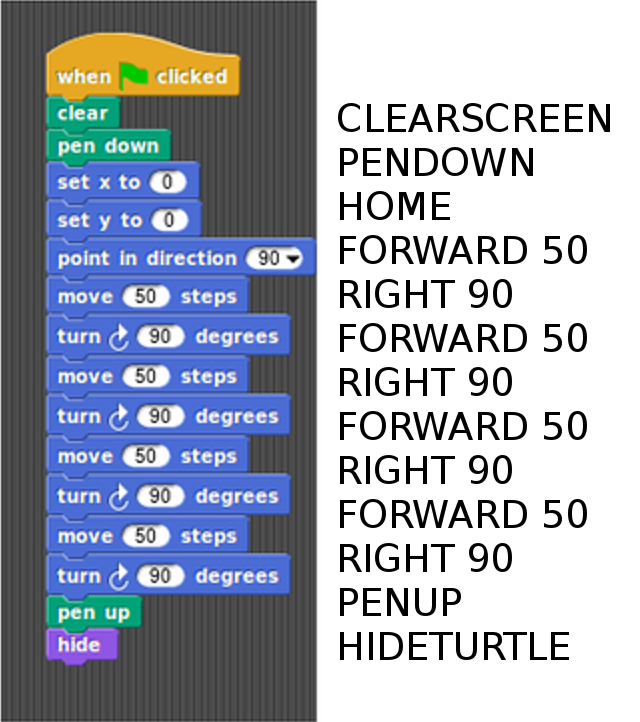
\includegraphics[width=7.5cm]{./images/librelogo/scratch-2.png}
   \label{scratch}
\end{figure}

Una caratteristica particolare di Scratch è quella di avere dato vita ad una vasta comunità di condivisione dei software. Questo è avvenuto grazie al fatto di essere stato concepito come un servizio web, che consente la composizione dei programmi e la possibilità di farli girare ma anche la realizzazione dell'aspetto \textit{social}, destinato alla condivisione e al riuso dei programmi. 
I linguaggi visuali non portano solo vantaggi. Sono (apparentemente) facili, divertenti e colorati, l'efficacia sembrerebbe garantita ma l'evidenza scientifica non è altrettanto chiara. Esistono infatti vari studi che mostrano come i linguaggi visuali non facilitino di fatto l'apprendimento dei linguaggi “veri” \cite{Weintrop}. 

Sembra che siano vantaggiosi per capire i più semplici costrutti della programmazione, questo sì, ma gli studi dove si testano le reali capacità di comprensione di quello che si ottiene con un certo codice non mostrano differenze sostanziali fra linguaggi visuali e testuali \cite{Weintrop2}. 

Particolarmente interessante è la ricerca di Colleen Lewis dove si confrontano i risultati ottenuti con Logo e con Scratch in una classe di bambini fra 10 e 12 anni \cite{Lewis}: se l'apprendimento di alcuni costrutti sembra facilitato da Scratch, non si sono osservate differenze nella percezione degli scolari che, anzi, hanno mostrato un livello di autostima superiore se introdotti alla programmazione con Logo. 

E anche se nelle fasi iniziali i giovani mostrano di gradire gli strumenti di tipo visuale, successivamente, una volta che sono entrati in contatto con la programmazione testuale convenzionale, talvolta sono loro stessi a denunciare i limiti del \textit{coding} visuale, per 1) la minore potenza, ovvero per i limiti imposti alla propria creatività, 2) per la maggiore lentezza nella programmazione quando questa si fa più complessa e 3) perché questi sistemi sono “meno veri”: “se devi fare una cosa vera nessuno ti chiederà mai di codificarla con un software didattico visuale” \cite{Weintrop3}.    

È sulla base di tali considerazioni che abbiamo deciso di approfondire il linguaggio Logo, quale strumento introduttivo alla programmazione. Di versioni di Logo oggi ce ne sono una quantità. Noi qui ci concentriamo su una versione che si trova normalmente nel programma di \textit{word} \textit{processing} Writer, incluso  nella suite per ufficio LibreOffice\footnote{Esiste un altro progetto analogo che si chiama OpenOffice. La domanda su quali siano le differenze rispetto a LibreOffice è molto frequente. Una piccola storia dell'evoluzione di questi due software, che hanno un origine comune, può essere trovata qui (luglio 2016): http://www.navigaweb.net/2014/04/differenze-tra-openoffice-e-libreoffice.html. Allo stato attuale, LibreOffice conviene perché incorpora più funzionalità e viene aggiornato più frequentemente.}, l'analogo del ben noto Microsoft Office. Quest'ultimo è un “prodotto proprietario”, vale a dire che l'azienda che lo produce lo vende ma senza distribuire il codice sorgente in chiaro, secondo il modello industriale convenzionale, con il quale la proprietà intellettuale è tenuta gelosamente segreta.  LibreOffice invece è software libero, e come tale è l'ideale per l'impiego in qualsiasi contesto formativo. In primo luogo perché comporta un messaggio di natura etica. Infatti il software libero è definito da quattro tipi di libertà: 1) libertà di eseguire il programma come si desidera, per qualsiasi scopo ; 2) libertà di studiare come funziona il programma e di modificarlo in modo da adattarlo alle proprie necessità; 3) libertà di ridistribuire copie in modo da aiutare il prossimo; 4) libertà di migliorare il programma e distribuirne pubblicamente i miglioramenti eventualmente apportati, in modo tale che tutta la comunità ne tragga beneficio. Poiché le libertà N. 2 e 4, per potere essere esercitate, richiedono la lettura del codice sorgente del software, va da se che il software libero, per essere tale, deve necessariamente rendere disponibile il codice sorgente. Occorre osservare – su questo punto molti fanno confusione – che il software di tipo \textit{open} \textit{source} non coincide con il software libero (\textit{free} \textit{software}) perché manca la connotazione etica: con il software open source si assume che il codice sorgente sia disponibile in chiaro, ma non si fa menzione delle suddette quattro libertà e, in particolare, delle due specificazioni che connotano la valenza etica del \textit{free} \textit{software}:  “in modo da aiutare il prossimo” nella terza libertà e “in modo tale che tutta la comunità ne tragga beneficio” nella quarta libertà. Il software libero è sviluppato da comunità che al più si aggregano in società non a fini di lucro. L'\textit{open} \textit{source} è sviluppato da attori economici privati che aderiscono al paradigma di sviluppo condiviso perché lo trovano adeguato alle proprie strategie di marketing: vi sono aziende che curano progetti \textit{open\textit{}} source a fianco dei tradizionali prodotti proprietari perché lo trovano conveniente per le proprie strategie di marketing. Le funzionalità di LibreOffice possono essere arricchite da numerosi \textit{plugin}, ovvero componenti che aggiungono le funzionalità più diverse. Ebbene, LibreLogo è uno di questi e, dalla versione 4.0 in poi, il plugin LibreLogo è incluso di \textit{default} \footnote{Di \textit{default} significa che questo è il comportamento normale. Coloro che utilizzano Linux (per Windows o Mac questo problema non c'è) devono prendere nota di quanto segue. Fino alla versione LibreOffice 4 esclusa, installare l'estensione di LibreOffice da http://extensions.libreoffice.org/extension-center/librelogo. Invece dalla versione 4 in poi, installare direttamente il pacchettolibreoffice-librelogo, con il comando \textit{sudo apt-get install libreoffice-librelogo}. Dopodiché occorre fare ripartire LibreOffice, qualora fosse già aperto. Quindi attivare la toolbar in View->Toolbars->Logo. Richiudere e rilanciare
} nel programma. Ma cosa significa usare Logo in un \textit{word} \textit{processor} come Writer, se questo è un normale word processor mentre Logo è un linguaggio per disegnare? Semplice: con il \textit{plugin} LibreLogo si possono produrre immagini che risultano integrate nel documento, come se fossero importate. È un'idea geniale, dovuta a Németh László, che ha riprodotto tutte le funzionalità di Logo all'interno di LibreOffice. In  realtà le ha ulteriormente incrementate, traendo vantaggio dal linguaggio Python, con cui ha scritto il plugin. Usare LibreLogo è semplicissimo: si apre un documento in Writer, si scrive un po' di codice in linguaggio Logo, come fosse un qualsiasi altro testo, e poi si esegue premendo l'apposito tasto nella \textit{toolbar} di LibreLogo; se il codice è corretto, la tartaruga esegue il disegno codificato nel testo in mezzo alla pagina. Successivamente, questo disegno può essere gestito e manipolato come qualsiasi altra grafica di LibreOffice. Quando si lancia LibreOffice, se non si è mai usato LibreLogo, la \textit{toolbar} di LibreLogo non è attiva. Occorre quindi attivarla, con l'appropriato comando di menu: \textbf{View} $\rightarrow$ \textbf{Toolbars} $\rightarrow$ \textbf{Logo}: 

\begin{figure}[h]
   \centering
   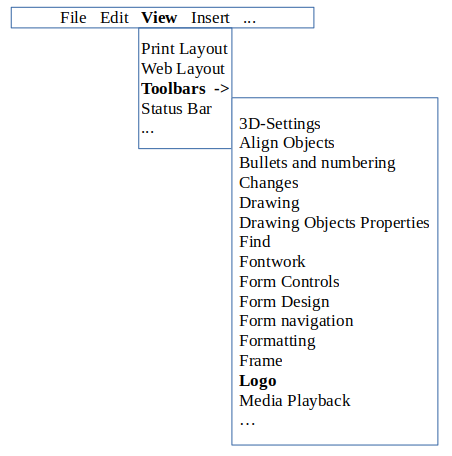
\includegraphics[width=7.5cm]{./images/librelogo/AttivazioneToolbar.png}
   \label{AttivazioneToolbar}
\end{figure}

Fatto questo, occorre chiudere il programma e rilanciarlo per vedere fra le altre \textit{toolbar} anche quella di LibreLogo. Questa appare nel seguente modo: 

\begin{figure}[h]
   \centering
   
\includegraphics[width=7.5cm]{./images/librelogo/LibreLogoToolbar.png}
   \label{LibreLogoToolbar}
\end{figure}

dove le icone hanno i seguenti significati:


\begin{center}
  \begin{tabular}{ c | l | p{5cm} }
    \hline
    
\includegraphics[width=0.75cm]{./images/librelogo/FrecciaSULO.png} & FORWARD 10 & Avanti di 10 punti (vedremo successivamente il significato dei punti) \\ \hline
    
\includegraphics[width=0.75cm]{./images/librelogo/FrecciagiuLO.png} & BACK 10 & Indietro di 10 punti \\ \hline
    
\includegraphics[width=0.75cm]{./images/librelogo/Orario.png} & LEFT 15 & A sinistra di -15 gradi \\ \hline
    
\includegraphics[width=0.75cm]{./images/librelogo/Antiorario.png} & RIGHT 15 & A destra di 15 gradi \\ \hline
    
\includegraphics[width=0.75cm]{./images/librelogo/PlayLO.png} &  & Esegue il programma scritto nel programma. Dalla versione 4.3 in poi, in un documento nuovo appena aperto esegue un programma di esempio. \\ \hline
    
\includegraphics[width=0.75cm]{./images/librelogo/StopLO.png} &  & Ferma il programma che sta girando (se dura troppo a lungo per qualche problema) \\ \hline
    
\includegraphics[width=0.75cm]{./images/librelogo/RewindLO.png} & HOME & Riporta Logo nella condizione iniziale, con la tartaruga al centro che punta in alto. \\ \hline
    
\includegraphics[width=0.75cm]{./images/librelogo/NewpageLO.png} & CLEARSCREEN & Cancella il disegno appena fatto (non il testo presente nel documento) \\ \hline
    
\includegraphics[width=0.75cm]{./images/librelogo/220px-TextLO.png} &  & Consente di scrivere un comando qualsiasi per eseguirlo subito
 \\ \hline
    
\includegraphics[width=0.75cm]{./images/librelogo/MagicwLO.png} &  & Aggiusta tutto il testo del programma rendendolo tutto maiuscolo. Traduce tutti i comandi nella lingua in cui è impostato LibreOffice. Al momento della revisione di queste note (agosto 2017) mi sono accorto che nei sorgenti di LibreLogo è stata impostata la lingua italiana ma il dizionario non è mai stato compilato. Mi riprometto di farlo appena possibile in modo che la modifica venga inserita nella revisione successiva di Libreoffice. \\ \hline
    \hline
  \end{tabular}
\end{center}

\section{La grafica di LibreLogo in Writer}

L'interazione fra LibreLogo e Writer è particolare per quanto riguarda la
grafica. All'inizio può sembrare farraginosa ma in realtà occorre abituarsi e
imparare due o tre regolette. La caratteristica, probabilmente unica, di
LibreLogo è che il risultato ottenuto girando\footnote{In gergo con “girare un
programma” si intende far funzionare un programma – in inglese to \textit{run a
program}. Oggi, con i moderni linguaggi spesso i programmi sono detti
\textit{script}. In generale un programma è un software completo e magari anche
molto complesso. Uno \textit{script} tende a essere un frammento di codice più
piccolo e specifico. Ma sono categorie che si sovrappongono largamente.} uno
script si ritrova sullo stesso supporto dove scriviamo il codice, ovvero un documento di tipo ODT di Writer. Di fatto in questo modo il documento ospita due tipi di informazioni diverse: una lista di istruzioni scritte in forma testuale e un oggetto grafico prodotto facendo funzionare quelle istruzioni. L'oggetto grafico è di tipo “vettoriale”, ovvero è composto da un insieme di oggetti geometrici. Altro sono le immagini tipo \textit{raster}, o \textit{bitmap}, che sono composte da una matrice di pixel\footnote{Un approfondimento della distinzione fra immagini bitmap e vettoriali può essere trovato in http://https://iamarf.org/2014/02/23/elaborazione-di-immagini-tre-fatti-che-fanno-la-differenza-loptis/}. Gli oggetti grafici prodotti da LibreLogo sono del tutto analoghi a quelli che prodotti con il tool di disegno a mano disponibile in Writer, accessibile attraverso l'apposita \textit{toolbar}, alla voce di menu \textbf{View} $\rightarrow$ \textbf{Toolbars} $\rightarrow$ \textbf{Drawing}: : 

\begin{figure}[h]
   \centering
   
\includegraphics[width=12.0cm]{./images/librelogo/DrawToolbar.png}
   \label{DrawToolbar}
\end{figure}

Come tali, i disegni fatti con LibreLogo possono essere spostati, copiati o salvati come qualsiasi altro oggetto grafico. Una cosa utile da capire è che spesso tali oggetti sono in realtà una composizione di oggetti distinti. In questo manuale ne faremo molti. Per utilizzarli come un unico oggetto occorre usare la funzione di raggruppamento, procedendo così: prima si delimita la regione che comprende gli oggetti da raggruppare, selezionando il \textit{pointer} 
\includegraphics[height=1em]{./images/librelogo/Pointer_LO.png} nella barra di disegno e poi delineando la regione rettangolare desiderata con il mouse e tenendo premuto il tasto sinistro. Attenzione che il cursore del mouse deve avere la forma della freccia e non quella tipica di quando si inserisce il testo, a forma di una I maiuscola, perché con questo si inserisce testo e non grafica. Il fatto che sia attivo il cursore grafico (e non testuale) si capisce anche dal fatto che contestualmente si attiva un'altra toolbar, che serve al controllo della grafica:

\begin{figure}[h]
   \centering
   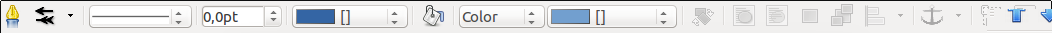
\includegraphics[width=12.0cm]{./images/librelogo/DrawToolbar2.png}
   \label{DrawToolbar2}
\end{figure}

Quando si seleziona la regione che contiene gli oggetti grafici, in questa barra si attivano alcune icone, fra cui quella della funzione raggruppamento: 
\includegraphics[height=1em]{./images/librelogo/RaggruppamentoLO.png}. Premendo questa tutti gli oggetti grafici compresi nella regione selezionata vengono raggruppati in un unico oggetto grafico che può essere copiato altrove o salvato. 

Un altro accorgimento utile è quello di “ancorare” appropriatamente la grafica al documento, laddove la dobbiamo usare. Sempre nella solita barra per la grafica, il tasto che consente di determinare l'ancoraggio è questa: 
\includegraphics[height=1em]{./images/librelogo/AncoraLO.png}. Cliccando sulla freccetta a sinistra dell'ancora si possono selezionare quattro tipi di ancoraggio: 1) “alla pagina”, 2) “al paragrafo”, 3) “al carattere” e 4) “come carattere”. Nel primo caso la grafica è associata alla pagina e non si muove da questa, nel secondo ad un paragrafo, nel terzo ad un carattere e nel quarto si comporta come se fosse un carattere. Quale sia l'ancoraggio più opportuno è una cosa che si impara con l'esperienza. La maggior parte delle grafiche in questo manuale sono state ancorate “al paragrafo”, eccetto che per le piccole immagini che stanno in linea con il testo, come l'ancora precedente, queste sono ancorate “come carattere”. 

Queste cose appena dette riguardano la gestione della grafica in Writer in generale. Usando LibreLogo, l'unica differenza è che la grafica viene prodotta attraverso le istruzioni che mettiamo nel codice. LibreLogo piazza la grafica nel mezzo della prima pagina del documento, anche se il testo del codice si dilunga nelle pagine successive. Può succedere così che la grafica si sovrapponga al testo del codice medesimo. Di primo acchito sembra che il comportamento sia farraginoso se non errato. Niente di tutto questo. La grafica è prodotta per essere usata da qualche parte. Si tratta semplicemente di selezionarla, con gli accorgimenti appena descritti e portata altrove, in una pagina pulita semplicemente per vederla con chiarezza, oppure in qualche altro documento dove questa debba essere integrata.


















